\tunemarkup{coverimage}{%
\newpagecolor{ubpagecolor}\afterpage{\restorepagecolor}
\tunemarkup{pghanlin}{\begin{center}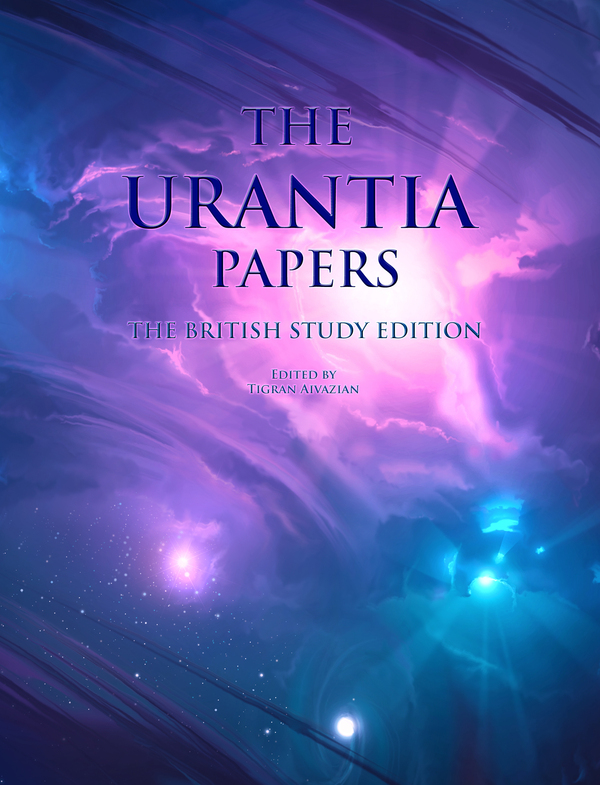
\includegraphics[scale=1.64]{images/British-Study-Edition-Cover-tiny.jpg}\end{center}}
\tunemarkup{pgkoboaurahd}{\begin{center}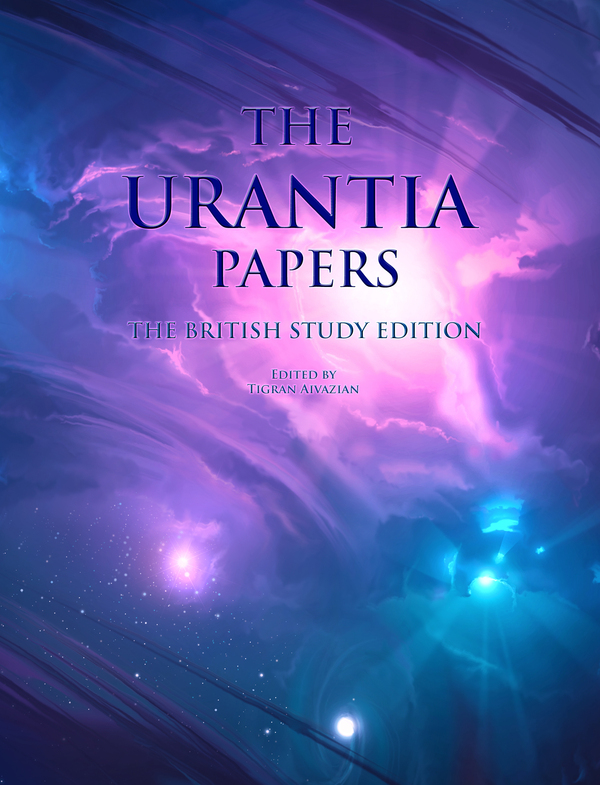
\includegraphics[scale=1.89]{images/British-Study-Edition-Cover-tiny.jpg}\end{center}}
\tunemarkup{pgnexus7}{\begin{center}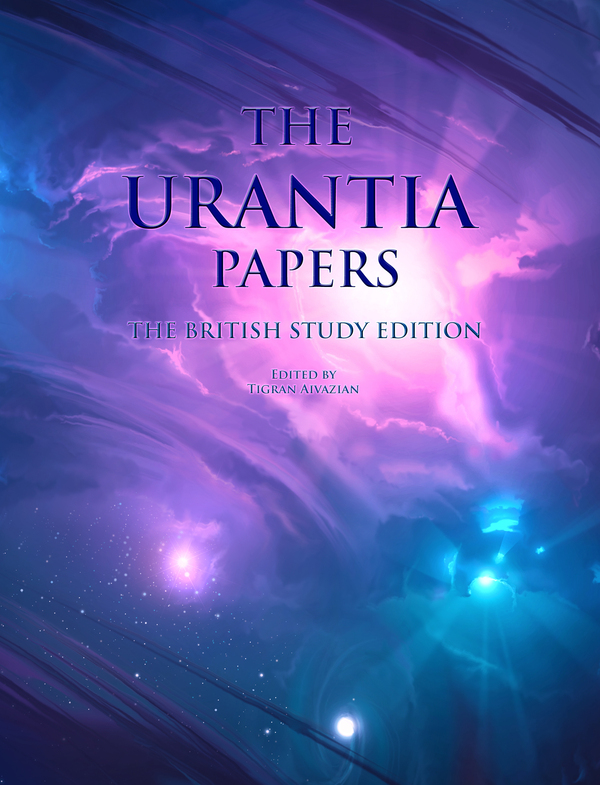
\includegraphics[scale=1.71]{images/British-Study-Edition-Cover-tiny.jpg}\end{center}}
\tunemarkup{pgkindledx}{\begin{center}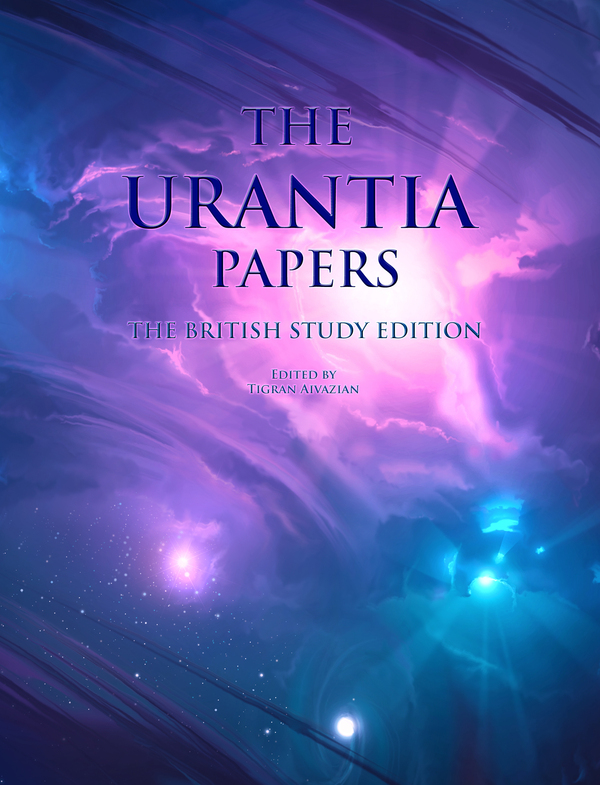
\includegraphics[scale=2.7]{images/British-Study-Edition-Cover-tiny.jpg}\end{center}}
\newpage
}

\makeatletter
\bib@raise@anchor{\bibpdfbookmark[0]{Title Page}{Ttl}}%
\makeatother

\vspace*{\stretch{0.01}}
\begin{center}
{
\bibcovertitlefont
\tunemarkup{pgkindledx}{\fontsize{18.2}{32}\selectfont}
\tunemarkup{pghanlin}{\fontsize{12}{20}\selectfont}
\tunemarkup{pgnexus7}{\fontsize{13.5}{20}\selectfont}
\tunemarkup{pgkoboaurahd}{\fontsize{15.5}{20}\selectfont}
THE BRITISH STUDY EDITION\\
\tunemarkup{pgkindledx}{\fontsize{16.5}{32}\selectfont}
\tunemarkup{pghanlin}{\fontsize{9}{20}\selectfont}
\tunemarkup{pgnexus7}{\fontsize{10}{20}\selectfont}
\tunemarkup{pgkoboaurahd}{\fontsize{12}{20}\selectfont}
{\itshape OF}\\[1ex]
\tunemarkup{pghanlin}{\fontsize{17}{20}\selectfont}
\tunemarkup{pgkindledx}{\fontsize{25}{32}\selectfont}
\tunemarkup{pgnexus7}{\fontsize{18.5}{20}\selectfont}
\tunemarkup{pgkoboaurahd}{\fontsize{21}{20}\selectfont}
\urantiabook\\
\tunemarkup{pgkindledx}{\fontsize{16.5}{32}\selectfont}
\tunemarkup{pghanlin}{\fontsize{9}{20}\selectfont}
\tunemarkup{pgnexus7}{\fontsize{10}{20}\selectfont}
\tunemarkup{pgkoboaurahd}{\fontsize{12}{20}\selectfont}
{\itshape ALSO KNOWN AS}\\[1ex]
\tunemarkup{pghanlin}{\fontsize{15}{20}\selectfont}
\tunemarkup{pgkindledx}{\fontsize{25}{32}\selectfont}
\tunemarkup{pgnexus7}{\fontsize{15}{20}\selectfont}
\tunemarkup{pgkoboaurahd}{\fontsize{18}{20}\selectfont}
``THE URANTIA BOOK''\\
}%
{%
\vspace*{\stretch{0.1}}
\tunemarkup{pghanlin}{\fontsize{10}{13}\selectfont}
\tunemarkup{pgkindledx}{\fontsize{16}{18}\selectfont}
\tunemarkup{pgnexus7}{\fontsize{10}{12}\selectfont}
\tunemarkup{pgkoboaurahd}{\fontsize{13}{15}\selectfont}
\itshape
The Standard Reference Text in British English\tunemarkuptwo{nofnt}{}{%
,\\
with Metric Measures, Textual Variants,\\
Study Notes \&\ \totalfigures\ Illustrations\\
}
\tunemarkup{pgnexus7}{\textcolor{ubdarkred}{With Words of Jesus in Red Colour}\\}
}%
\vspace*{\stretch{0.6}}
\tunemarkuptwo{nofancydecor}{}{%
\titlesepbig\\
}
\vspace*{\stretch{0.1}}
\end{center}

\tunemarkuptwo{nofancydecor}{}{\titleframe}

\newpage
\makeatletter
\bib@raise@anchor{\bibpdfbookmark[0]{Copyright Page}{Cpr}}%
\makeatother

\begin{center}
\vspace*{\stretch{0.3}}
\tunemarkup{pghanlin}{\begin{center}\parbox{7cm}{\normalsize\bfseries\itshape ``Of all human knowledge, that which is of greatest value is to know the religious life of Jesus and how he lived it.'' \bibref[(196:1.3)]{p196 1:3}}\end{center}}
\tunemarkup{pgnexus7}{\begin{center}\parbox{7cm}{\normalsize\bfseries\itshape ``Of all human knowledge, that which is of greatest value is to know the religious life of Jesus and how he lived it.'' \bibref[(196:1.3)]{p196 1:3}}\end{center}}
\tunemarkup{pgkindledx}{\begin{center}\parbox{9cm}{\large\bfseries\itshape ``Of all human knowledge, that which is of greatest value is to know the religious life of Jesus and how he lived it.'' \bibref[(196:1.3)]{p196 1:3}}\end{center}}
\vspace*{\stretch{0.5}}
\tunemarkup{pghanlin}{\fontsize{8}{10}\itshape}
\tunemarkup{pgnexus7}{\fontsize{8}{10}\itshape}
\tunemarkup{pgkindledx}{\fontsize{10}{12}\itshape}
\parbox{0.9\linewidth}{\centering
\textbf{\upshape\nocopyright\ No copyright is claimed on this edition.\\The text of the Urantia Papers is in the \itshape public domain}.\\[5pt]
Cover design by Gary Tonge, www.vision-afar.com.\\
The latest version of this book can be downloaded from:\\
{\upshape\bfseries http://www.bibles.org.uk}\\
%The apparatus (marked with a circle in the text) contains all significant changes made since the 1955 first edition of the Urantia Book.\\
The symbol \pc\tunemarkup{pgluluhb}{\kern-2pt} marks the first paragraph in the group as in the first edition, where such groups were delimited by blank lines.\\
%The asterisk * indicates a study note other than a textual variant.\\[5pt]
\tux\ Typeset with \XeLaTeX\ under Linux.\\
Text set in \textbf{\tunemarkup{minionpro}{Adobe }\tunemarkup{garamond}{Adobe }\urantiamainfont} at \urantiamainfontsize pt.\\[18pt]
\upshape\small\bfseries Version: \mytoday{}\\
}
\end{center}

\tunemarkuptwo{nofancydecor}{}{\titleframe}
